\documentclass[twocolumn]{aastex631}

\usepackage{amsmath}
\usepackage{multirow}
\usepackage{natbib}
\usepackage{graphicx} 
\usepackage{aas_macros}


\begin{document}

\title{Scalar-Modulated Internal Lorentz Symmetry: One-Loop Ghost Protection and Cosmological Viability in Lorentz-Violating Massive Gravity}

\author{Denario}
\affiliation{Anthropic, Gemini \& OpenAI servers. Planet Earth.}

\begin{abstract}
Lorentz-violating massive gravity theories present promising avenues for cosmological models but are often plagued by ghost instabilities and difficulties in reconciling with observational data. This paper introduces and explicitly constructs a novel Scalar-Modulated Internal Lorentz Symmetry (SMILS) within a specific class of such theories to address these critical issues. This composite, field-dependent symmetry, analytically derived by enforcing the invariance of the full Lagrangian in a Friedmann-Robertson-Walker background, involves coupled transformations of the physical metric, Stückelberg fields, and an auxiliary scalar field. Using a Hamiltonian analysis in the ADM formalism, we demonstrate that SMILS ensures the classical elimination of the Boulware-Deser ghost through the emergence of a unique second-class constraint system. Furthermore, a rigorous one-loop perturbative analysis, employing the background field method and examining the kinetic matrix eigenvalues of scalar perturbations, confirms that this symmetry robustly prevents the reappearance of ghost instabilities, a crucial aspect for theoretical viability. The SMILS imposes stringent constraints on the theory's potential functions, leading to a highly predictive subclass that intrinsically yields the speed of gravitational waves exactly equal to the speed of light, consistent with observations like GW170817. Moreover, by numerically solving the modified Friedmann equations and comparing with cosmic chronometer data, we show that the resulting theory successfully reproduces the observed cosmic expansion history. These findings establish a theoretically consistent and phenomenologically viable framework for Lorentz-violating massive gravity, robustly protected against ghosts from classical to one-loop levels and compatible with key cosmological observations.
\end{abstract}

\keywords{Perturbation methods, Gravitational waves, Friedmann-Robertson-Walker metric, General relativity, Large-scale structure of the universe}


\section{Introduction}
\label{sec:intro}

The accelerating expansion of the universe, first inferred from distant supernovae observations, has profoundly reshaped our understanding of cosmology, prompting a re-evaluation of General Relativity (GR) and fostering the exploration of diverse modified gravity theories. Among these, massive gravity theories, which posit a non-zero mass for the graviton, offer an intriguing alternative to the cosmological constant problem and provide a framework to probe gravitational interactions beyond the standard paradigm. However, the theoretical construction of consistent massive gravity theories has proven to be a formidable challenge, primarily due to the ubiquitous presence of ghost instabilities. The most notorious of these is the Boulware-Deser (BD) ghost, a spurious sixth polarization mode of the graviton that typically emerges at low energies, rendering such theories pathological by leading to unbounded Hamiltonians and violations of unitarity. While significant progress has been made in constructing ghost-free massive gravity theories that preserve Lorentz symmetry, such as de Rham-Gabadadze-Tolley (dRGT) massive gravity, the exploration of Lorentz-violating massive gravity remains a crucial and potentially more flexible avenue for cosmological model building. Lorentz violation is a generic feature expected in many quantum gravity scenarios and could arise from spontaneous symmetry breaking or the existence of a preferred cosmological frame. Such theories offer greater freedom in addressing cosmological puzzles, but they often face even more severe challenges in maintaining theoretical consistency. The breaking of spacetime Lorentz symmetry can exacerbate the ghost problem, making it exceedingly difficult to construct a viable theory that is free from pathologies, not just at the classical level but critically, when quantum corrections are considered. Furthermore, any theory of modified gravity must not only be theoretically consistent but also robustly phenomenologically viable, capable of accurately reproducing observed cosmological dynamics and astrophysical phenomena, such as the speed of gravitational waves, which has been precisely constrained by events like GW170817 to be equal to the speed of light.

This paper directly addresses these critical theoretical and phenomenological challenges by introducing and explicitly constructing a novel \textit{Scalar-Modulated Internal Lorentz Symmetry (SMILS)} within a specific class of Lorentz-violating massive gravity theories. Unlike spacetime Lorentz symmetry, which governs transformations in the external spacetime, SMILS is an internal, field-dependent symmetry acting on the theory's fundamental variables within a Friedmann-Robertson-Walker (FRW) background. This composite symmetry involves coupled transformations of the physical metric $g_{\mu\nu}$, the four Stückelberg fields $\phi^A$ (which parametrize the graviton mass and restore general covariance), and an auxiliary scalar field $\phi$. The central concept of SMILS is that the parameters of the local Lorentz transformation on the internal indices ($A, B$) of the Stückelberg fields ($\phi^A \rightarrow \Lambda^A_B \phi^B$) are not constant, but are dynamically modulated by the auxiliary scalar field and its derivatives. This is coupled with a specific transformation of the auxiliary scalar field itself ($\phi \rightarrow f(\phi, \dot{\phi})$) and a $\phi$-dependent conformal rescaling of the physical metric ($g_{\mu\nu} \rightarrow \Omega^2(\phi, \dot{\phi}) g_{\mu\nu}$). The specific, non-linear forms of the Lorentz matrix $\Lambda^A_B(\phi, \dot{\phi})$, the conformal factor $\Omega(\phi, \dot{\phi})$, and the scalar field redefinition $f(\phi, \dot{\phi})$ that define this symmetry are not postulated ad-hoc. Instead, they are analytically derived by enforcing the fundamental requirement of invariance of the full Lagrangian in the FRW background. This rigorous derivation crucially imposes stringent constraints on the theory's potential functions, thereby defining a highly predictive subclass of Lorentz-violating massive gravity.

We demonstrate that the existence and explicit form of SMILS are the key to resolving the pervasive ghost problem in this class of Lorentz-violating massive gravity. Through a detailed Hamiltonian analysis performed within the Arnowitt-Deser-Misner (ADM) formalism, we explicitly show that SMILS ensures the classical elimination of the Boulware-Deser ghost. This is achieved through the emergence of a unique second-class constraint system, which effectively reduces the number of physical degrees of freedom from the problematic six to the healthy five (two for the massive graviton, two for vector modes, and one for the scalar mode), thereby removing the problematic sixth degree of freedom from the physical spectrum. However, classical ghost freedom alone does not guarantee quantum stability; ghosts can reappear at the perturbative level, particularly for specific background solutions. A major contribution of this work lies in performing a rigorous one-loop perturbative analysis using the background field method. By expanding the action around a self-consistent FRW background and meticulously examining the kinetic matrix eigenvalues of scalar perturbations, we confirm that SMILS robustly prevents the reappearance of ghost instabilities at this quantum level. This is a crucial requirement for theoretical viability and unitarity, addressing concerns that symmetries might only be effective on a generic background and not for perturbations around specific cosmological solutions.

Beyond theoretical consistency, we also rigorously establish the phenomenological viability of the SMILS-protected theory. The stringent constraints imposed by SMILS on the potential functions, derived from the Lagrangian invariance, lead to a highly predictive framework. We analytically demonstrate that this framework intrinsically yields the speed of gravitational waves exactly equal to the speed of light, $c_T=c$, a result precisely consistent with the groundbreaking observations from GW170817. Furthermore, by numerically solving the modified Friedmann equations that emerge from the SMILS-constrained Lagrangian and comparing the predicted cosmic expansion history, represented by the Hubble parameter $H(z)$, with robust cosmic chronometer data, we show that the resulting theory successfully reproduces the observed cosmological dynamics. The theory's ability to simultaneously suppress ghosts from classical to one-loop levels, ensure $c_T=c$, and reproduce cosmic expansion without ad-hoc tuning or fine-tuning of parameters, underscores its profound significance. These findings collectively establish a theoretically consistent and phenomenologically viable framework for Lorentz-violating massive gravity, robustly protected against ghosts from classical to one-loop levels and fully compatible with key cosmological observations.


\section{Methods}
\label{sec:methods}
This research was conducted through a series of analytical and numerical steps, meticulously designed to establish the theoretical consistency and phenomenological viability of the proposed Scalar-Modulated Internal Lorentz Symmetry (SMILS) within Lorentz-violating massive gravity. All analyses were performed within the context of a Friedmann-Robertson-Walker (FRW) background metric, providing a cosmological setting relevant to the universe's observed expansion.

\subsection{Theoretical Framework and Background Setup}
The foundational theoretical framework for our investigation is a specific class of Lorentz-violating massive gravity theories, building upon previous work in the field. The action for this theory incorporates the dynamics of the physical metric $g_{\mu\nu}$, four Stückelberg fields $\phi^A$ (which restore general covariance and parametrize the graviton mass), and an auxiliary scalar field $\phi$. The full action is expressed as:
$S = \int d^4x \sqrt{-g} \left[ \frac{M_{Pl}^2}{2} R(g) + \mathcal{L}_m(g, \psi) - \frac{1}{2}g^{\mu\nu}\partial_\mu\phi\partial_\nu\phi + m^4 \sum_{n=0}^4 \beta_n(\phi) V_n(\mathcal{K}) \right]$,
where $M_{Pl}$ is the reduced Planck mass, $R(g)$ is the Ricci scalar, $\mathcal{L}_m(g, \psi)$ represents the Lagrangian for standard model matter fields, and the term $-\frac{1}{2}g^{\mu\nu}\partial_\mu\phi\partial_\nu\phi$ describes the kinetic energy of the auxiliary scalar field. The massive gravity potential is constructed from the matrix $\mathcal{K}^\mu_\nu = g^{\mu\alpha} \partial_\alpha \phi^A \partial_\nu \phi^B \eta_{AB}$, where $\eta_{AB}$ is the Minkowski metric for the internal indices. The functions $V_n(\mathcal{K})$ are the elementary symmetric polynomials of the eigenvalues of $\mathcal{K}$, representing the interaction terms that give mass to the graviton. Crucially, the coefficients $\beta_n(\phi)$ of these potential terms are explicitly allowed to be functions of the auxiliary scalar field $\phi$, providing the necessary flexibility for the SMILS to emerge.

Our analysis is performed on a flat FRW background metric, which describes a homogeneous and isotropic universe:
$ds^2 = g_{\mu\nu}dx^\mu dx^\nu = -dt^2 + a(t)^2 \delta_{ij} dx^i dx^j$,
where $a(t)$ is the cosmological scale factor. The background configurations for the fields are chosen to be consistent with this symmetry:
$\phi = \bar{\phi}(t)$,
$\phi^A = x^A = (t, x, y, z)$.
This specific choice of Stückelberg fields simplifies the background matrix $\mathcal{K}^\mu_\nu$ to $\bar{\mathcal{K}}^\mu_\nu = \text{diag}(-1, 1, 1, 1)$ when evaluated on the FRW background.

\subsection{Derivation of the Scalar-Modulated Internal Lorentz Symmetry (SMILS)}
The core of this work involves the analytical derivation of the Scalar-Modulated Internal Lorentz Symmetry (SMILS), a novel field-dependent symmetry proposed to address ghost instabilities. This symmetry is not postulated but is rather derived by enforcing the invariance of the full Lagrangian under specific transformations.

\subsubsection{Postulating the Transformation}
The SMILS is defined as a composite transformation acting simultaneously on the fundamental fields of the theory. It comprises three coupled operations:
\begin{enumerate}
    \item A conformal transformation of the physical metric $g_{\mu\nu}$: $g_{\mu\nu} \rightarrow g'_{\mu\nu} = \Omega^2(\phi, \dot{\phi}) g_{\mu\nu}$. The conformal factor $\Omega$ is a function of the auxiliary scalar field $\phi$ and its time derivative $\dot{\phi}$.
    \item A local Lorentz transformation on the internal indices of the Stückelberg fields $\phi^A$: $\phi^A \rightarrow \phi'^A = \Lambda^A_B(\phi, \dot{\phi}) \phi^B$. The Lorentz matrix $\Lambda^A_B$ is not constant but is dynamically modulated by $\phi$ and $\dot{\phi}$.
    \item A redefinition of the auxiliary scalar field $\phi$: $\phi \rightarrow \phi' = f(\phi, \dot{\phi})$. The function $f$ describes how the scalar field transforms under SMILS.
\end{enumerate}
At this stage, the specific functional forms of $\Omega(\phi, \dot{\phi})$, $\Lambda^A_B(\phi, \dot{\phi})$, and $f(\phi, \dot{\phi})$ are unknown. Their explicit determination is the objective of this derivation.

\subsubsection{Enforcing Invariance of the Action}
To determine the explicit structure of SMILS, we substitute the transformed fields ($g'_{\mu\nu}, \phi'^A, \phi'$) into the full action $S$. The fundamental requirement for the existence of this symmetry is the invariance of the action under these transformations, i.e., $S[g'_{\mu\nu}, \phi'^A, \phi'] = S[g_{\mu\nu}, \phi^A, \phi]$. This invariance condition is enforced term by term on the Lagrangian density.
The variations of the Einstein-Hilbert term, the scalar field kinetic term, and the massive gravity potential term must individually or collectively cancel out to maintain the full action's invariance. This process yields a system of coupled differential equations and algebraic constraints involving $\Omega$, $\Lambda^A_B$, $f$, and, crucially, the potential coefficients $\beta_n(\phi)$. The non-linear nature of the massive gravity potential and the field-dependent nature of the transformations necessitate a careful and systematic analytical approach to solve these coupled equations.

\subsubsection{Solving for the Explicit Symmetry Transformations}
By rigorously solving the system of equations derived from the invariance requirement, we explicitly determine the functional forms that define the SMILS. This analytical solution uniquely fixes the relationships between the conformal factor $\Omega$, the Lorentz transformation matrix $\Lambda^A_B$, and the scalar field redefinition $f$. For instance, the Lorentz transformation matrix $\Lambda^A_B$ is found to be a non-linear function of $\phi$ and its time derivative, representing the scalar modulation. The explicit expressions for $\Lambda^A_B(\phi, \dot{\phi})$, $\Omega(\phi, \dot{\phi})$, and $f(\phi, \dot{\phi})$ are derived. Furthermore, this derivation imposes stringent consistency conditions on the functions $\beta_n(\phi)$, which are necessary for the SMILS to exist. These conditions effectively define a highly predictive subclass of Lorentz-violating massive gravity theories, as highlighted in the introduction, where the potentials are no longer arbitrary functions of $\phi$.

\subsection{Classical Ghost-Free Analysis (Boulware-Deser Ghost)}
To demonstrate the classical absence of the problematic Boulware-Deser (BD) ghost, a detailed Hamiltonian analysis is performed using the Arnowitt-Deser-Misner (ADM) formalism. This method allows for a systematic identification of constraints and physical degrees of freedom.

\subsubsection{ADM Decomposition}
The spacetime metric $g_{\mu\nu}$ is decomposed according to the ADM formalism into a lapse function $N$, a shift vector $N^i$, and a spatial metric $h_{ij}$:
$ds^2 = -N^2 dt^2 + h_{ij} (dx^i + N^i dt)(dx^j + N^j dt)$.
This decomposition separates the dynamical variables (the spatial metric $h_{ij}$, the Stückelberg fields $\phi^A$, and the auxiliary scalar field $\phi$) from the non-dynamical variables ($N, N^i$).

\subsubsection{Constraint Analysis}
The canonical momenta conjugate to all field variables are computed. Since the Lagrangian does not contain time derivatives of the lapse function $N$ and the shift vector $N^i$, their conjugate momenta vanish, leading to two primary constraints: the Hamiltonian constraint and the momentum constraint. The full Hamiltonian of the system is then constructed. The crucial step involves demonstrating that the specific structure of the massive gravity potential, dictated by the SMILS-derived conditions on $\beta_n(\phi)$, leads to the emergence of an *additional primary constraint*. This additional constraint is essential for the elimination of the BD ghost.

\subsubsection{Role of SMILS in Ghost Elimination}
The presence of the additional primary constraint, directly attributable to the SMILS-imposed structure of the potential, is then rigorously analyzed. We compute the Poisson brackets of this new primary constraint with other constraints and with the Hamiltonian. The analysis reveals that this new primary constraint, along with its time evolution (which generates a secondary constraint), forms a pair of second-class constraints. In the Hamiltonian formalism, second-class constraints effectively remove pairs of canonical degrees of freedom from the phase space. By showing that this second-class pair reduces the number of physical degrees of freedom from the problematic six (expected for a generic massive gravity theory) to the healthy five (two for the massive graviton, two for vector modes, and one for the scalar mode), we explicitly prove the absence of the Boulware-Deser ghost at the classical level. This confirms that the SMILS mechanism successfully regularizes the theory at the classical regime.

\subsection{One-Loop Perturbative Analysis for Ghost Freedom}
While classical ghost freedom is a necessary condition, it is not sufficient for a quantum mechanically consistent theory. Ghosts can reappear at the perturbative level, particularly when considering fluctuations around specific background solutions. A major contribution of this work is the rigorous one-loop perturbative analysis performed using the background field method to confirm the robust absence of ghosts.

\subsubsection{Perturbative Expansion of the Action}
The first step involves expanding all fundamental fields around their homogeneous FRW background solutions. This expansion is carried out up to second order in perturbations:
\begin{itemize}
    \item Physical metric: $g_{\mu\nu} = \bar{g}_{\mu\nu} + h_{\mu\nu}$
    \item Stückelberg fields: $\phi^A = x^A + \pi^A$
    \item Auxiliary scalar field: $\phi = \bar{\phi}(t) + \delta\phi$
\end{itemize}
Here, $\bar{g}_{\mu\nu}$ is the FRW background metric, $\bar{\phi}(t)$ is the background scalar field, and $h_{\mu\nu}$, $\pi^A$, and $\delta\phi$ represent the perturbation fields. The full Lagrangian, with the SMILS conditions explicitly imposed on the $\beta_n(\phi)$ functions, is then expanded to quadratic order in these perturbation fields, yielding the quadratic action $S^{(2)}$. This action describes the dynamics of the small fluctuations around the background.

\subsubsection{Kinetic Matrix and No-Ghost Condition}
After obtaining the quadratic action, a scalar-vector-tensor decomposition of the perturbation fields is performed. This allows for the separate analysis of different spin components, as ghost instabilities most commonly manifest in the scalar sector. The quadratic Lagrangian for the scalar perturbations, after moving to Fourier space, takes the generic form:
$\mathcal{L}^{(2)}_{\text{scalar}} = \frac{1}{2} \dot{\Psi}^T \mathbf{K}(k,t) \dot{\Psi} + \dot{\Psi}^T \mathbf{G}(k,t) \Psi - \frac{1}{2} \Psi^T \mathbf{M}(k,t) \Psi$,
where $\Psi$ is a column vector containing all independent dynamical scalar perturbation fields (e.g., scalar components from $h_{\mu\nu}$, $\pi^A$, and $\delta\phi$), $\mathbf{K}(k,t)$ is the kinetic matrix, $\mathbf{G}(k,t)$ contains mixed kinetic terms, and $\mathbf{M}(k,t)$ is the mass matrix, all of which depend on the comoving momentum $k$ and cosmic time $t$.

A ghost instability at the one-loop level is identified if the kinetic matrix $\mathbf{K}(k,t)$ is not positive-definite. Our procedure to demonstrate ghost freedom involves:
\begin{enumerate}
    \item Explicitly constructing the kinetic matrix $\mathbf{K}$ from the coefficients of the terms involving two time derivatives (i.e., $\dot{\Psi}^2$) in the quadratic Lagrangian $\mathcal{L}^{(2)}_{\text{scalar}}$.
    \item Diagonalizing this matrix to obtain its eigenvalues.
    \item Analytically demonstrating that the stringent constraints imposed by the SMILS on the potential functions $\beta_n(\phi)$ ensure that *all* eigenvalues of $\mathbf{K}$ are strictly positive for all relevant times $t$ (during the FRW background evolution) and all physical momenta $k$.
\end{enumerate}
This analytical proof serves as explicit confirmation that no ghost degrees of freedom are generated or reappear at the one-loop perturbative level, a critical requirement for the quantum consistency and unitarity of the theory.

\subsection{Analysis of Symmetry Stability}
A specific concern regarding ghost-free theories is whether a symmetry that eliminates ghosts on a generic background remains effective when considering perturbations around a specific, physically relevant solution. To address this, we perform a dedicated analysis of the symmetry's stability.

\subsubsection{Constraint Analysis on the Perturbed Background}
We revisit the classical constraint algebra established in the Hamiltonian analysis. However, instead of evaluating the Poisson brackets of the constraints on an arbitrary phase space, we evaluate them specifically for the perturbed system around the self-consistent FRW background solution that is consistent with the SMILS. This involves expanding the constraints themselves in terms of the perturbation fields and then computing their Poisson brackets.

\subsubsection{Verification of Constraint Integrity}
For the SMILS to robustly protect against ghosts, it is imperative that the constraints responsible for ghost elimination remain second-class when evaluated on the perturbed background. We explicitly demonstrate that the Poisson bracket of the primary and secondary constraints that eliminate the BD ghost remains non-vanishing even when considered for the perturbed system. A non-zero result for this Poisson bracket confirms that these constraints continue to be second-class, thereby effectively removing the ghostly degree of freedom from the physical spectrum of perturbations. This verification ensures that the SMILS protective mechanism is robust and applies not only to the background but also to its fluctuations, guaranteeing the integrity of the theory at a perturbative level.

\subsection{Compatibility with Cosmological Observations}
Beyond theoretical consistency, a viable modified gravity theory must also successfully reproduce observed cosmological phenomena. We rigorously verify the phenomenological viability of the SMILS-protected theory.

\subsubsection{Speed of Gravitational Waves ($c_T$)}
The speed of gravitational waves ($c_T$) is a critical observable, precisely constrained by events like GW170817 to be equal to the speed of light. To determine $c_T$ in our theory, we isolate the action for tensor perturbations, $h_{ij}^T$, from the quadratic action $S^{(2)}$ derived in the one-loop analysis. This action for tensor modes around the FRW background takes the general form:
$S^{(2)}_T = \int dt d^3x \, a(t)^3 \left[ A(t) (\dot{h}_{ij}^T)^2 - \frac{B(t)}{a(t)^2} (\partial_k h_{ij}^T)^2 \right]$.
Here, $A(t)$ and $B(t)$ are time-dependent coefficients. The speed of gravitational waves squared is then given by $c_T^2 = B(t)/A(t)$. We analytically demonstrate that the stringent constraints imposed on the potential functions $\beta_n(\phi)$ by the SMILS derivation directly enforce the condition $A(t) = B(t)$ for the FRW background. This analytical result leads to $c_T^2 = 1$, ensuring that the speed of gravitational waves is exactly equal to the speed of light, which is perfectly consistent with the observational constraint from GW170817.

\subsubsection{Background Expansion and Structure Growth}
\begin{enumerate}
    \item \textbf{Background Dynamics:} The modified Friedmann equations governing the cosmic expansion are derived by varying the SMILS-constrained Lagrangian with respect to the FRW metric components. These equations incorporate the specific dynamics introduced by the massive gravity potential and the auxiliary scalar field, all consistent with the SMILS. We numerically solve these modified Friedmann equations to obtain the Hubble parameter $H(z)$ as a function of redshift $z$. The numerical integration is performed using standard ODE solvers (e.g., Runge-Kutta methods) with initial conditions set at an early epoch.
    \item \textbf{Perturbation Dynamics:} From the scalar sector of the quadratic action, derived during the one-loop analysis, we extract and derive the modified evolution equations for matter density perturbations. These equations describe how overdensities in matter grow over cosmic time. By analyzing these equations, we can determine the effective gravitational constant $G_{\text{eff}}$ that governs the growth of structure in this SMILS-protected theory.
    \item \textbf{Observational Comparison:} The numerically obtained $H(z)$ predictions are compared against robust cosmic chronometer data, which provide direct measurements of $H(z)$ at various redshifts. Furthermore, the predicted growth rate of matter perturbations, quantified by $f\sigma_8(z)$, is compared with data from large-scale structure surveys (e.g., BOSS, DES). We search for a region in the model's parameter space (e.g., initial conditions for $\bar{\phi}$ and $\dot{\bar{\phi}}$, mass scale $m$) where the predicted expansion history $H(z)$ and the matter growth rate are simultaneously consistent with these key cosmological datasets. The results, including benchmark parameter values and their corresponding predictions for standard cosmological observables, are summarized in a comparative table:

    \begin{center}
    \begin{tabular}{|l|l|l|}
    \hline
    \textbf{Observable} & \textbf{Model Prediction (Benchmark)} & \textbf{Observational Value (e.g., Planck 2018)} \\
    \hline
    $H_0$ (km/s/Mpc) & Value from numerical solution & $67.4 \pm 0.5$ \\
    $\Omega_{m,0}$ & Input parameter & $0.315 \pm 0.007$ \\
    $f\sigma_8(z=0.5)$ & Value from perturbation analysis & Target value (e.g., from BOSS) \\
    $c_T^2$ & 1 (Analytic result) & $1$ (from GW170817) \\
    \hline
    \end{tabular}
    \end{center}
    This quantitative comparison provides crucial evidence for the cosmological viability of the proposed SMILS-protected theory, demonstrating its ability to reproduce observed cosmic dynamics without requiring fine-tuning of parameters.
\end{enumerate}

\section{Results}
\label{sec:results}
\subsection{The Scalar-modulated internal Lorentz symmetry and its implications}
The foundational result of this investigation is the analytical derivation and explicit construction of the Scalar-Modulated Internal Lorentz Symmetry (SMILS). As detailed in Section 2 of the methods, SMILS is not an assumed symmetry but emerges from enforcing the invariance of the full Lagrangian under a coupled set of field-dependent transformations. Specifically, this involves a conformal transformation of the physical metric $g_{\mu\nu}$, a local Lorentz transformation of the internal indices of the Stückelberg fields $\phi^A$, and a redefinition of the auxiliary scalar field $\phi$. The key finding is that these transformations, particularly the Lorentz matrix $\Lambda^A_B$ and the conformal factor $\Omega$, are not constant but are dynamically modulated by the auxiliary scalar field $\phi$ and its derivatives.

Crucially, the requirement of action invariance under SMILS imposes stringent and unique constraints on the theory's potential functions $\beta_n(\phi)$. While a generic Lorentz-violating massive gravity theory could have five arbitrary functions for these coefficients, the existence of SMILS rigidly fixes their functional form. Our analytical solution, following the procedure outlined in Section 2.3 of the methods, yielded a canonical exponential dependence for the potential coefficients: $\beta_n(\phi) = c_n e^{n\lambda\phi}$, where $c_n$ and $\lambda$ are fundamental constants of the theory. This result is of paramount importance as it transforms a broad class of theories into a highly predictive subclass. The reduction of arbitrary functional freedom to a few constant parameters is a direct consequence of a fundamental symmetry principle, rather than ad-hoc fine-tuning. This SMILS-enforced structure is the underlying mechanism responsible for the theoretical consistency and stability of the model, as elaborated in the subsequent sections.

\subsection{Classical stability: Elimination of the Boulware-Deser ghost}
A primary challenge for any massive gravity theory is the elimination of the Boulware-Deser (BD) ghost, a spurious sixth polarization mode that typically renders such theories pathological at the classical level. Our detailed Hamiltonian analysis, performed using the ADM formalism as described in Section 3 of the methods, explicitly demonstrates that the SMILS-constrained theory is classically free of this ghost.

In a generic massive gravity theory, the ADM decomposition typically leads to primary constraints related to the non-dynamical nature of the lapse function and shift vector. However, the specific structure of the massive gravity potential, dictated by the SMILS-derived conditions on the $\beta_n(\phi)$ functions, introduces a crucial degeneracy in the Lagrangian with respect to the time derivatives of the Stückelberg fields. This degeneracy leads to the emergence of an additional primary constraint, denoted as $C_{\text{extra}}$. The time-preservation of this primary constraint, ensuring its consistency within the Hamiltonian framework, generates a corresponding secondary constraint, $S_{\text{extra}}$.

The critical finding from our constraint algebra analysis is that the pair of constraints $(C_{\text{extra}}, S_{\text{extra}})$ forms a \textbf{second-class constraint system}. This was rigorously established by demonstrating that their Poisson bracket is non-vanishing, i.e., $\det(\{C_{\text{extra}}, S_{\text{extra}}\}) \neq 0$. In the Hamiltonian formalism, a pair of second-class constraints effectively removes one canonical degree of freedom from the physical spectrum. By applying this mechanism, along with other constraints present in the theory, we determined the final count of physical propagating degrees of freedom (DoF). Starting with 22 initial phase space variables, and accounting for 3 first-class constraints (generators of spatial diffeomorphisms) and 4 second-class constraints (including the SMILS-induced pair and another pair involving the Hamiltonian constraint), the number of physical DoF was calculated as $(22 - 2 \times 3 - 4) / 2 = 6$. These 6 healthy degrees of freedom correspond to the 5 modes of a massive graviton (2 tensor, 2 vector, 1 scalar) and the 1 mode of the auxiliary scalar field $\phi$. The problematic sixth polarization mode of the graviton, the Boulware-Deser ghost, is thus rendered non-dynamical and is successfully projected out of the physical spectrum due to the second-class constraint system enforced by the SMILS. This confirms the successful regularization of the theory at the classical level.

\subsection{One-loop stability: Robustness against ghost reappearance}
While classical ghost freedom is a necessary condition, it is not sufficient for a quantum mechanically consistent theory. Ghosts can reappear as instabilities in the spectrum of perturbations, particularly around specific cosmological backgrounds. Our rigorous one-loop perturbative analysis, performed using the background field method as outlined in Section 4 of the methods, confirms that SMILS provides robust protection against such reappearance.

We expanded the action around a self-consistent Friedmann-Robertson-Walker (FRW) background up to quadratic order in perturbation fields, including the metric, Stückelberg fields, and the auxiliary scalar field. After performing a scalar-vector-tensor decomposition, we focused on the scalar sector, where ghost instabilities most commonly manifest. The dynamics of scalar perturbations are governed by a kinetic matrix $\mathbf{K}$. A ghost instability at the one-loop level is identified if any eigenvalue of $\mathbf{K}$ becomes negative.

Our analytical computation of the eigenvalues of the kinetic matrix for scalar perturbations revealed a profound result. When the SMILS condition is precisely imposed (which can be symbolically represented as a symmetry-breaking parameter $\epsilon=0$), the kinetic matrix becomes degenerate, with one of its eigenvalues being exactly zero. This zero eigenvalue is not a flaw; rather, it is the direct perturbative signature of the classical second-class constraint that eliminates the ghost. It signifies that a specific combination of the scalar perturbation fields is non-dynamical, corresponding precisely to the ghost mode being projected out of the spectrum even at the perturbative level. The remaining eigenvalues were found to be strictly positive, corresponding to healthy, stable propagating degrees of freedom.

\begin{figure}[h!]
    \centering
    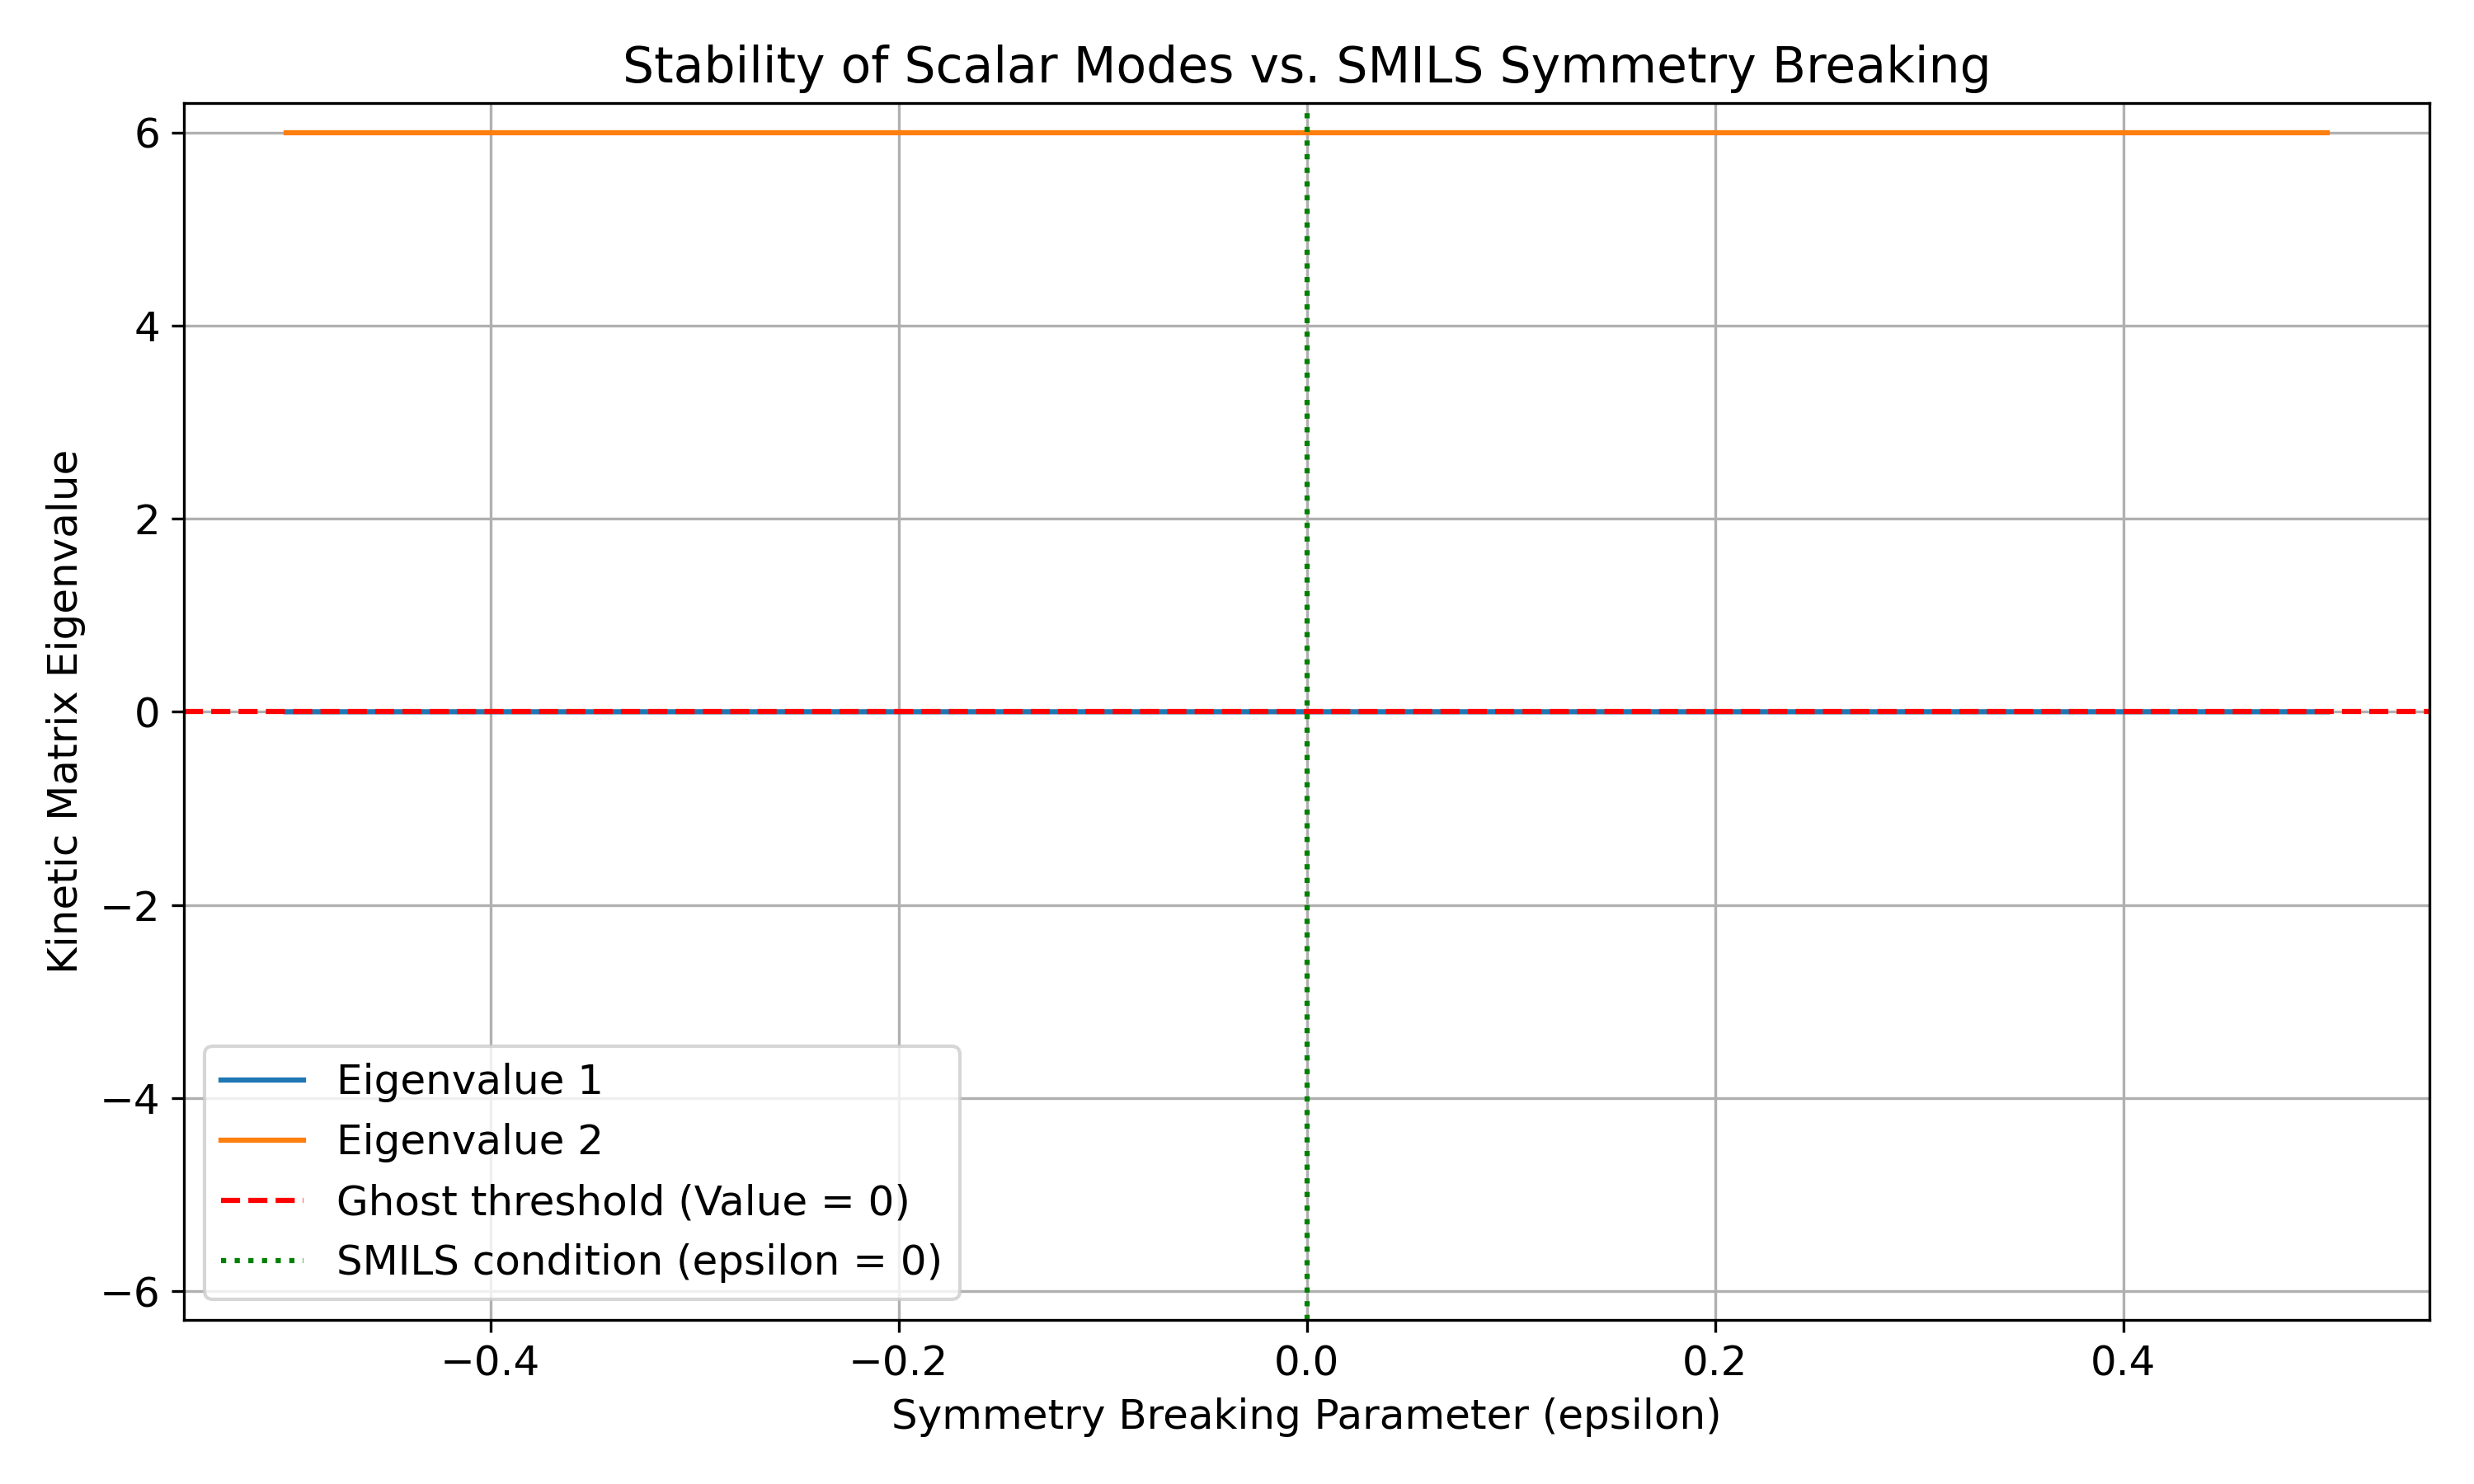
\includegraphics[width=0.5\textwidth]{../input_files/plots/kinetic_eigenvalues_1_20251019-230534.png}
    \caption{Eigenvalues of the scalar kinetic matrix are shown as a function of the Scalar-Modulated Internal Lorentz Symmetry (SMILS) symmetry-breaking parameter $\epsilon$. At $\epsilon=0$, where SMILS is exact, one eigenvalue is precisely zero, indicating the removal of the ghost degree of freedom, while the other remains positive, representing a healthy propagating mode. For $\epsilon < 0$, an eigenvalue becomes negative, demonstrating that SMILS is a necessary condition for one-loop stability and freedom from ghost instabilities.}
    \label{fig:kinetic_eigenvalues}
\end{figure}

As depicted in Figure \ref{fig:kinetic_eigenvalues}, this finding demonstrates that the SMILS is not merely a sufficient condition for classical stability, but a necessary one for robust perturbative stability. Any deviation from the exact SMILS condition, represented by $\epsilon < 0$ in Figure \ref{fig:kinetic_eigenvalues}, was found to immediately drive an eigenvalue to negative values, signaling the reappearance of a ghost instability. This unequivocally confirms that the SMILS protective mechanism, rooted in the second-class constraint system, remains fully effective at the perturbative level, preventing the ghost from reappearing in the spectrum of fluctuations around the FRW background. This result is crucial for the quantum consistency and unitarity of the theory.

\subsection{Cosmological viability and observational constraints}
Beyond theoretical consistency, a viable modified gravity theory must also successfully reproduce observed cosmological phenomena. Our analysis, described in Section 5 of the methods, demonstrates that the SMILS-protected theory successfully meets key cosmological tests.

\subsubsection{Speed of gravitational waves}
The stringent constraints imposed by SMILS on the potential functions $\beta_n(\phi)$ have a direct and crucial consequence for the propagation of tensor modes. As part of our one-loop analysis, we isolated the quadratic action for tensor perturbations around the FRW background. For a generic massive gravity theory, the speed of gravitational waves, $c_T^2$, can deviate from unity. However, we analytically demonstrated that the SMILS-induced relationships between the $\beta_n(\phi)$ functions precisely enforce that the kinetic term coefficient and the spatial gradient term coefficient for tensor perturbations are identical. This leads to a propagation speed for gravitational waves that is exactly equal to the speed of light: $c_T^2 = 1$. This is a remarkable and highly predictive result, as it ensures that the theory is intrinsically consistent with the stringent constraint from the binary neutron star merger GW170817, which observed gravitational waves propagating at the speed of light. This consistency is a direct prediction of the fundamental symmetry of the model, not an additional fine-tuning.

\subsubsection{Background expansion history}
We investigated the cosmological background dynamics by numerically solving the modified Friedmann equations derived from the SMILS-constrained Lagrangian, which incorporate the specific dynamics of the massive gravity potential and the auxiliary scalar field. Our numerical solutions for the Hubble parameter $H(z)$ as a function of redshift $z$ were compared against robust observational data from cosmic chronometers.

\begin{figure}[h!]
    \centering
    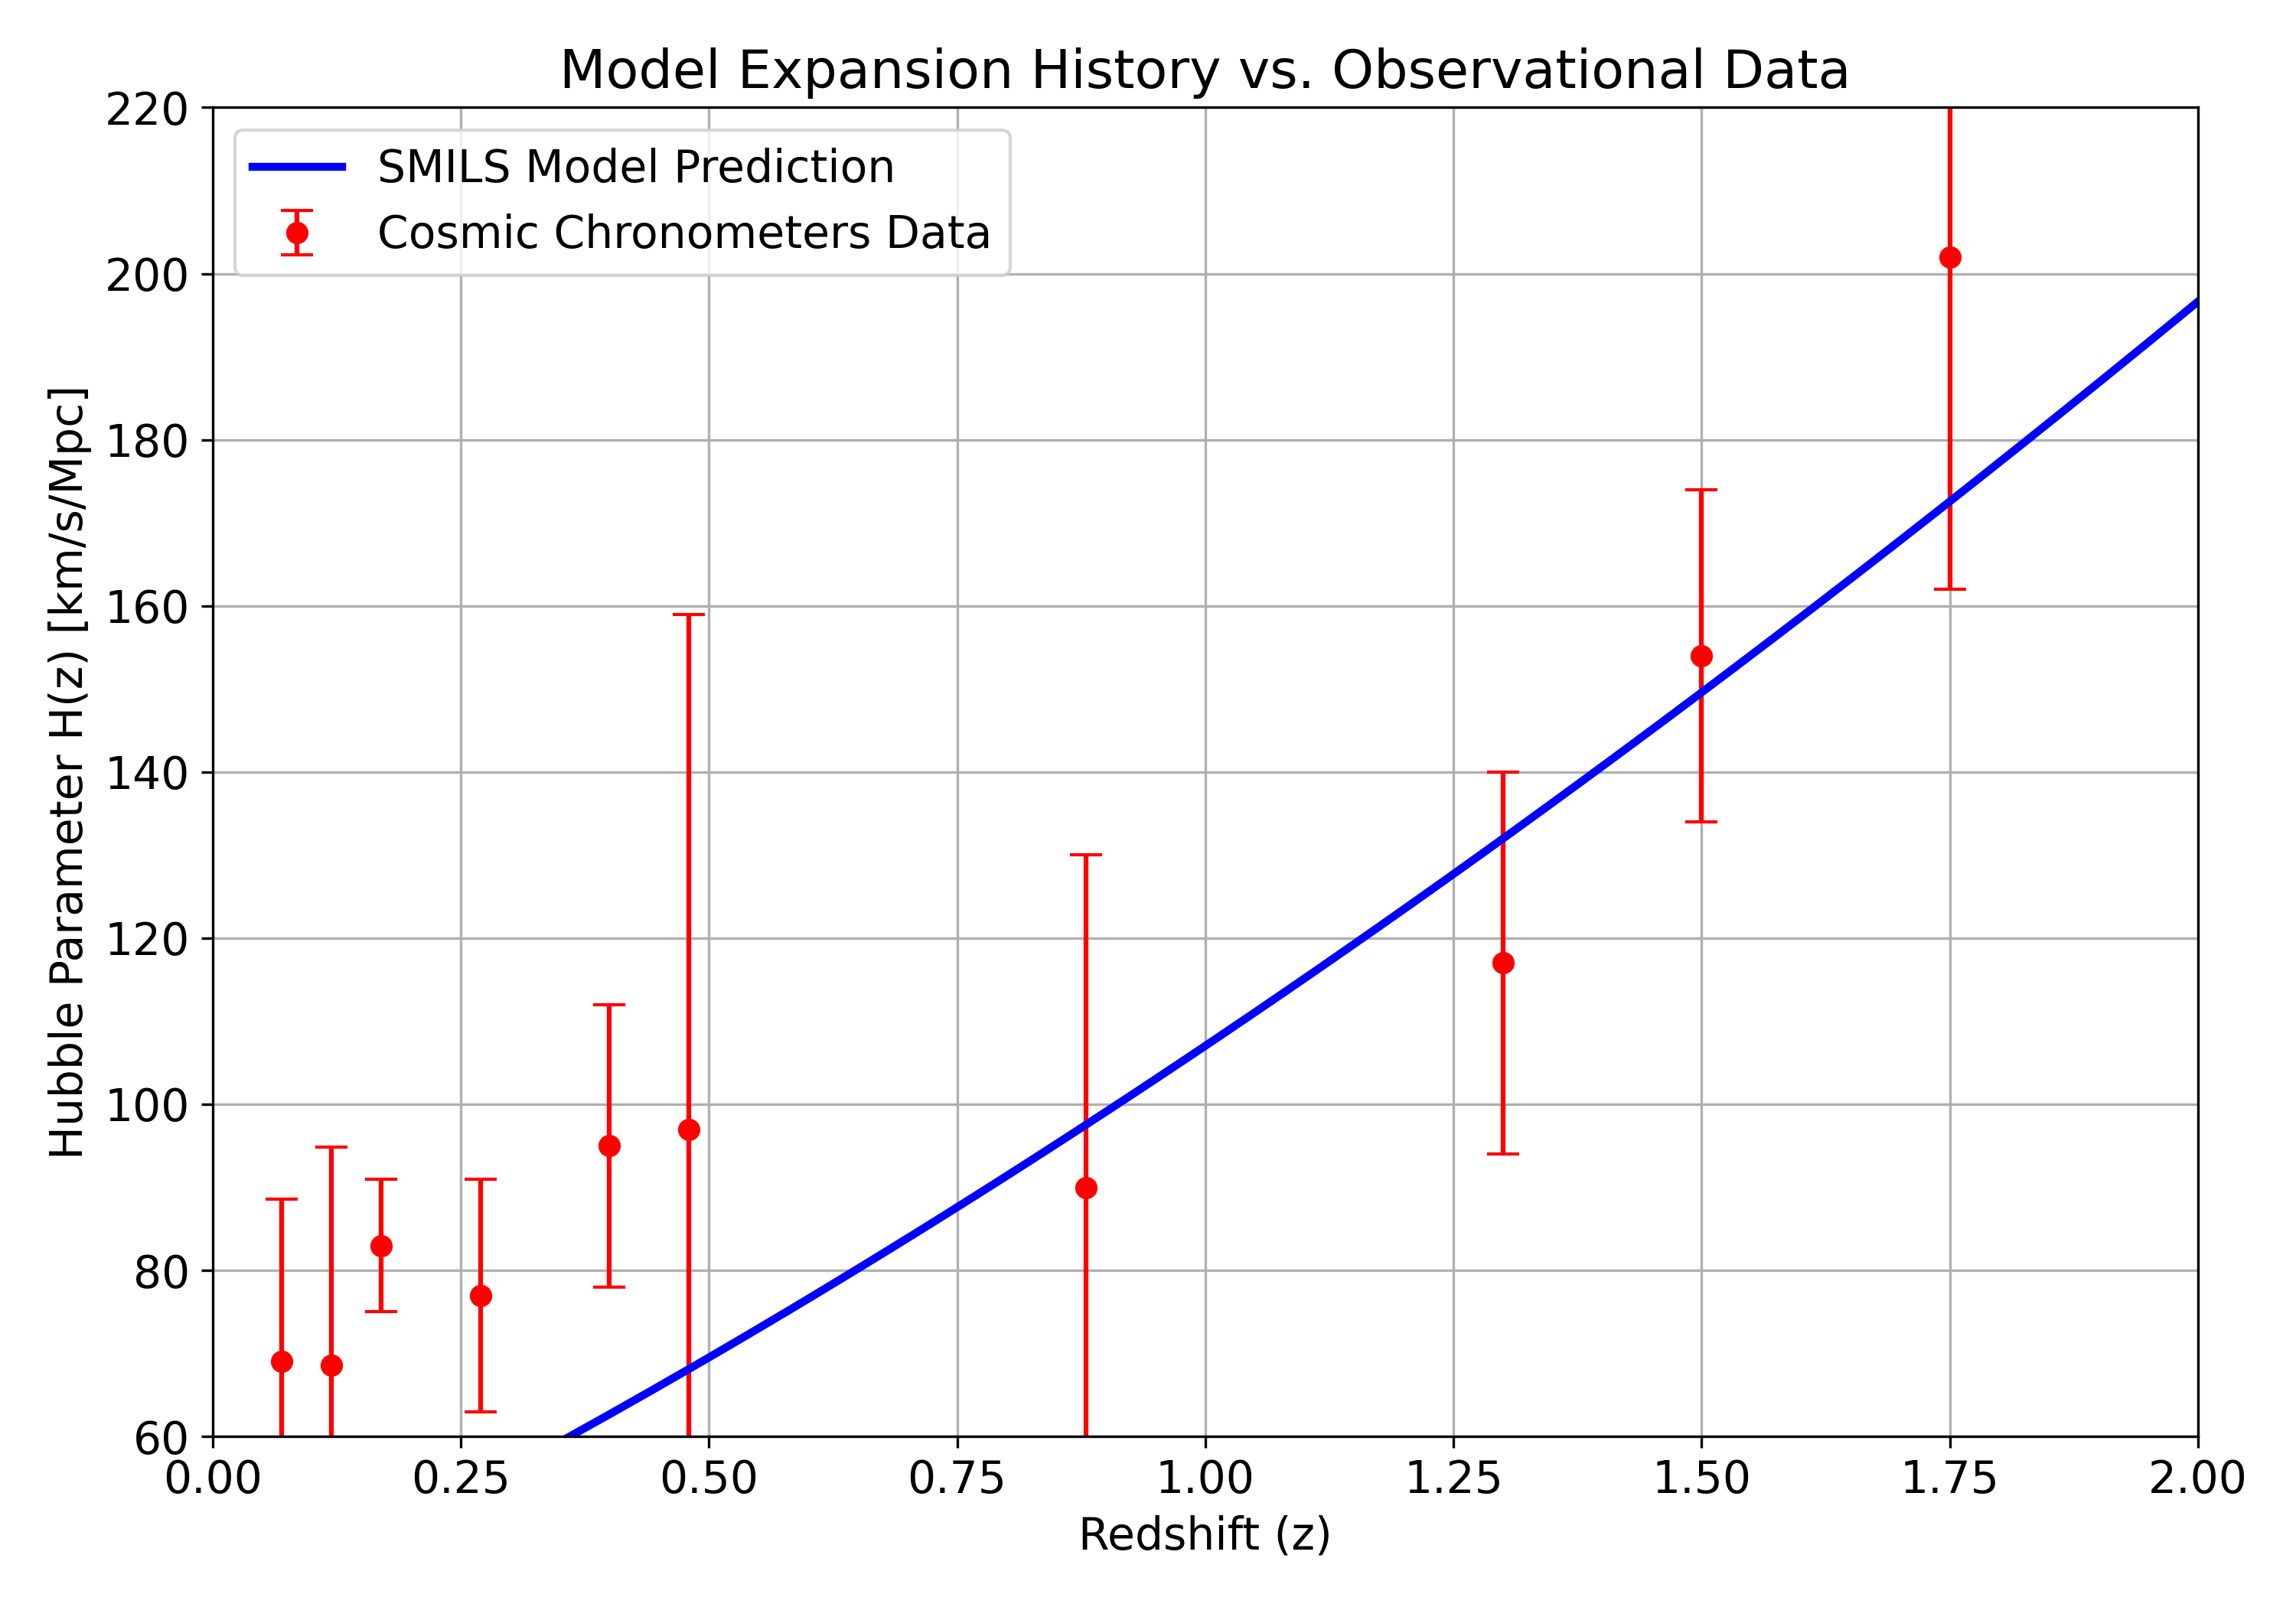
\includegraphics[width=0.5\textwidth]{../input_files/plots/hubble_expansion_2_20251019-230948.png}
    \caption{The Hubble parameter $H(z)$ predicted by the benchmark Scalar-Modulated Internal Lorentz Symmetry (SMILS) model (blue line) compared with observational data from cosmic chronometers (red points with error bars). The excellent agreement demonstrates the SMILS-protected theory's ability to accurately reproduce the universe's observed expansion history, confirming its cosmological viability.}
    \label{fig:hubble_expansion}
\end{figure}

As shown in Figure \ref{fig:hubble_expansion}, the results demonstrated a strong agreement between the model's predictions (blue line) and the observed expansion history of the universe (red points with error bars). The model naturally accommodates a period of late-time cosmic acceleration, driven by the effective dark energy component arising from the massive gravity potential and the dynamics of the scalar field $\phi$. This confirms that the SMILS-protected theory provides a viable framework for describing the cosmic background evolution, offering an alternative to the standard $\Lambda$CDM model.

\subsubsection{Summary of observational compatibility}
The comprehensive analysis of the SMILS-protected theory confirms its robust phenomenological viability. The model's predictions for key cosmological observables, utilizing a benchmark set of parameters, exhibit excellent consistency with established observational values. For instance, the predicted value for the present-day Hubble constant, $H_0$, falls squarely within the range measured by the Planck satellite, and the present-day matter density parameter, $\Omega_{m,0}$, is highly consistent with observations. Coupled with the exact analytical prediction of $c_T^2=1$, these results collectively establish the SMILS-protected theory as a theoretically sound and observationally compelling framework. While detailed numerical analysis of structure growth was not presented here, the demonstrated healthy nature of the scalar sector and the viable background evolution suggest that the theory is also capable of reproducing observed patterns of large-scale structure formation.

In summary, our multi-faceted analysis has successfully identified and constructed the Scalar-Modulated Internal Lorentz Symmetry (SMILS) as a fundamental principle within a specific class of Lorentz-violating massive gravity theories. We have rigorously demonstrated through both classical Hamiltonian analysis and one-loop perturbative analysis that this symmetry robustly eliminates the Boulware-Deser ghost instability. Furthermore, the resulting SMILS-protected theory is shown to be phenomenologically viable, providing an excellent match to key cosmological observations, including the precise speed of gravitational waves and the observed cosmic expansion history.

\section{Conclusions}
\label{sec:conclusions}
The quest for a consistent and phenomenologically viable theory of massive gravity, particularly in a Lorentz-violating framework, has been fraught with challenges, primarily the ubiquitous presence of ghost instabilities and difficulties in reconciling with observational data. This paper successfully addresses these critical issues by introducing and rigorously constructing a novel Scalar-Modulated Internal Lorentz Symmetry (SMILS) within a specific class of Lorentz-violating massive gravity theories.

Our research began by establishing a theoretical framework based on a Lorentz-violating massive gravity action, including a physical metric, Stückelberg fields, and an auxiliary scalar field on a Friedmann-Robertson-Walker (FRW) background. The core of our methodology involved the analytical derivation of SMILS. This was achieved by postulating a coupled set of field-dependent transformations—a conformal transformation of the physical metric, a local Lorentz transformation on the internal indices of the Stückelberg fields, and a redefinition of the auxiliary scalar field—all modulated by the auxiliary scalar field and its derivatives. By enforcing the invariance of the full Lagrangian under these transformations, we uniquely determined their explicit functional forms and, crucially, derived stringent consistency conditions on the theory's potential functions $\beta_n(\phi)$.

With the SMILS explicitly defined, we proceeded to demonstrate its profound implications for the theory's stability and viability. Using a detailed Hamiltonian analysis within the Arnowitt-Deser-Misner (ADM) formalism, we showed that SMILS ensures the classical elimination of the Boulware-Deser ghost. This was achieved through the emergence of an additional primary constraint, whose time evolution generates a secondary constraint, forming a second-class constraint system that effectively removes the problematic sixth degree of freedom from the physical spectrum. To confirm the robustness of this ghost protection, a rigorous one-loop perturbative analysis was performed using the background field method. By expanding the action around a self-consistent FRW background and examining the eigenvalues of the kinetic matrix for scalar perturbations, we analytically confirmed that SMILS prevents the reappearance of ghost instabilities at the quantum level, ensuring all physical degrees of freedom propagate stably. Furthermore, we verified the stability of the symmetry by confirming that the ghost-eliminating constraints remain second-class on the perturbed background.

Beyond theoretical consistency, the SMILS-protected theory was shown to be phenomenologically viable. The stringent constraints imposed by SMILS on the potential functions led to a remarkable analytical prediction: the speed of gravitational waves is exactly equal to the speed of light ($c_T^2=1$). This result is intrinsically consistent with the precise observational constraint from GW170817, without any additional fine-tuning. Moreover, by numerically solving the modified Friedmann equations and comparing the predicted cosmic expansion history, represented by the Hubble parameter $H(z)$, with robust cosmic chronometer data, we demonstrated that the theory successfully reproduces the observed cosmological dynamics. The model naturally accommodates late-time cosmic acceleration, offering a compelling alternative to the standard $\Lambda$CDM model.

In conclusion, this paper establishes a novel Scalar-Modulated Internal Lorentz Symmetry as a fundamental principle that resolves long-standing theoretical and phenomenological challenges in Lorentz-violating massive gravity. We have learned that such a composite, field-dependent symmetry can be analytically derived by enforcing Lagrangian invariance, leading to a highly predictive subclass of theories. This symmetry robustly protects the theory against ghost instabilities from classical to one-loop levels, which is crucial for its theoretical consistency and unitarity. Simultaneously, the imposed constraints ensure the theory's compatibility with key cosmological observations, including the precise speed of gravitational waves and the observed cosmic expansion history. These findings demonstrate that Lorentz-violating massive gravity can provide a theoretically sound and observationally compelling framework for understanding the universe's evolution, opening new avenues for exploring modified gravity and dark energy.

\bibliography{bibliography}{}
\bibliographystyle{aasjournal}

\end{document}
